%!TEX program = xelatex
% Note: this template must be compiled with XeLaTeX rather than PDFLaTeX
% due to the custom fonts used. The line above should ensure this happens
% automatically, but if it doesn't, your LaTeX editor should have a simple toggle
% to switch to using XeLaTeX.

\documentclass[
  aspectratio=169, % Uncomment to use an aspect ratio of 16:9 (160 mm by 90 mm)
  %aspectratio=43, % Uncomment to use an aspect ratio of 4:3 (128mm by 96mm)
  t, % Top align all slide content by default
  onlytextwidth, % Typeset content in columns at text width
  10pt, % Default font size, use 10pt for the 16:9 aspect ratio and 8pt for the 4:3 aspect ratio
]{beamer}

\usepackage{../../ImperialTheme/beamer/beamerthemeImperial} % Use the Imperial theme

\def\imagefolder{../../ImperialTheme/beamer/Images}
\def\Rey{\text{Re}}
\title{n factor} % Presentation title to appear on the title slide and left footers

\subtitle{} % Presentation subtitle to appear on the title slide

\author{Víctor Ballester} % Author name(s) to appear on the title slide

\date{\today} % Presentation date to appear on the title slide and right footers

\begin{document}

\begingroup
\setbeamercolor{background canvas}{bg=ICLBlue} % Slide background color
\setbeamercolor{title page title}{fg=white} % Title text color
\setbeamercolor{title page subtitle}{fg=white} % Subtitle text color
\setbeamercolor{author}{fg=white} % Author(s) text color
\setbeamercolor{date}{fg=white} % Date text color
\setbeamertemplate{title page}[logo]{\imagefolder/ICL_Logo_White.pdf} % Imperial logo color, use 'ICL_Logo_White.pdf' for white and 'ICL_Logo_Blue.pdf' for blue
\frame[plain, s]{\titlepage} % Output the title page with no footer ('plain') and vertically distributed text ('s')
\endgroup

\begin{frame}
	\frametitle{Recap}
	\centering
	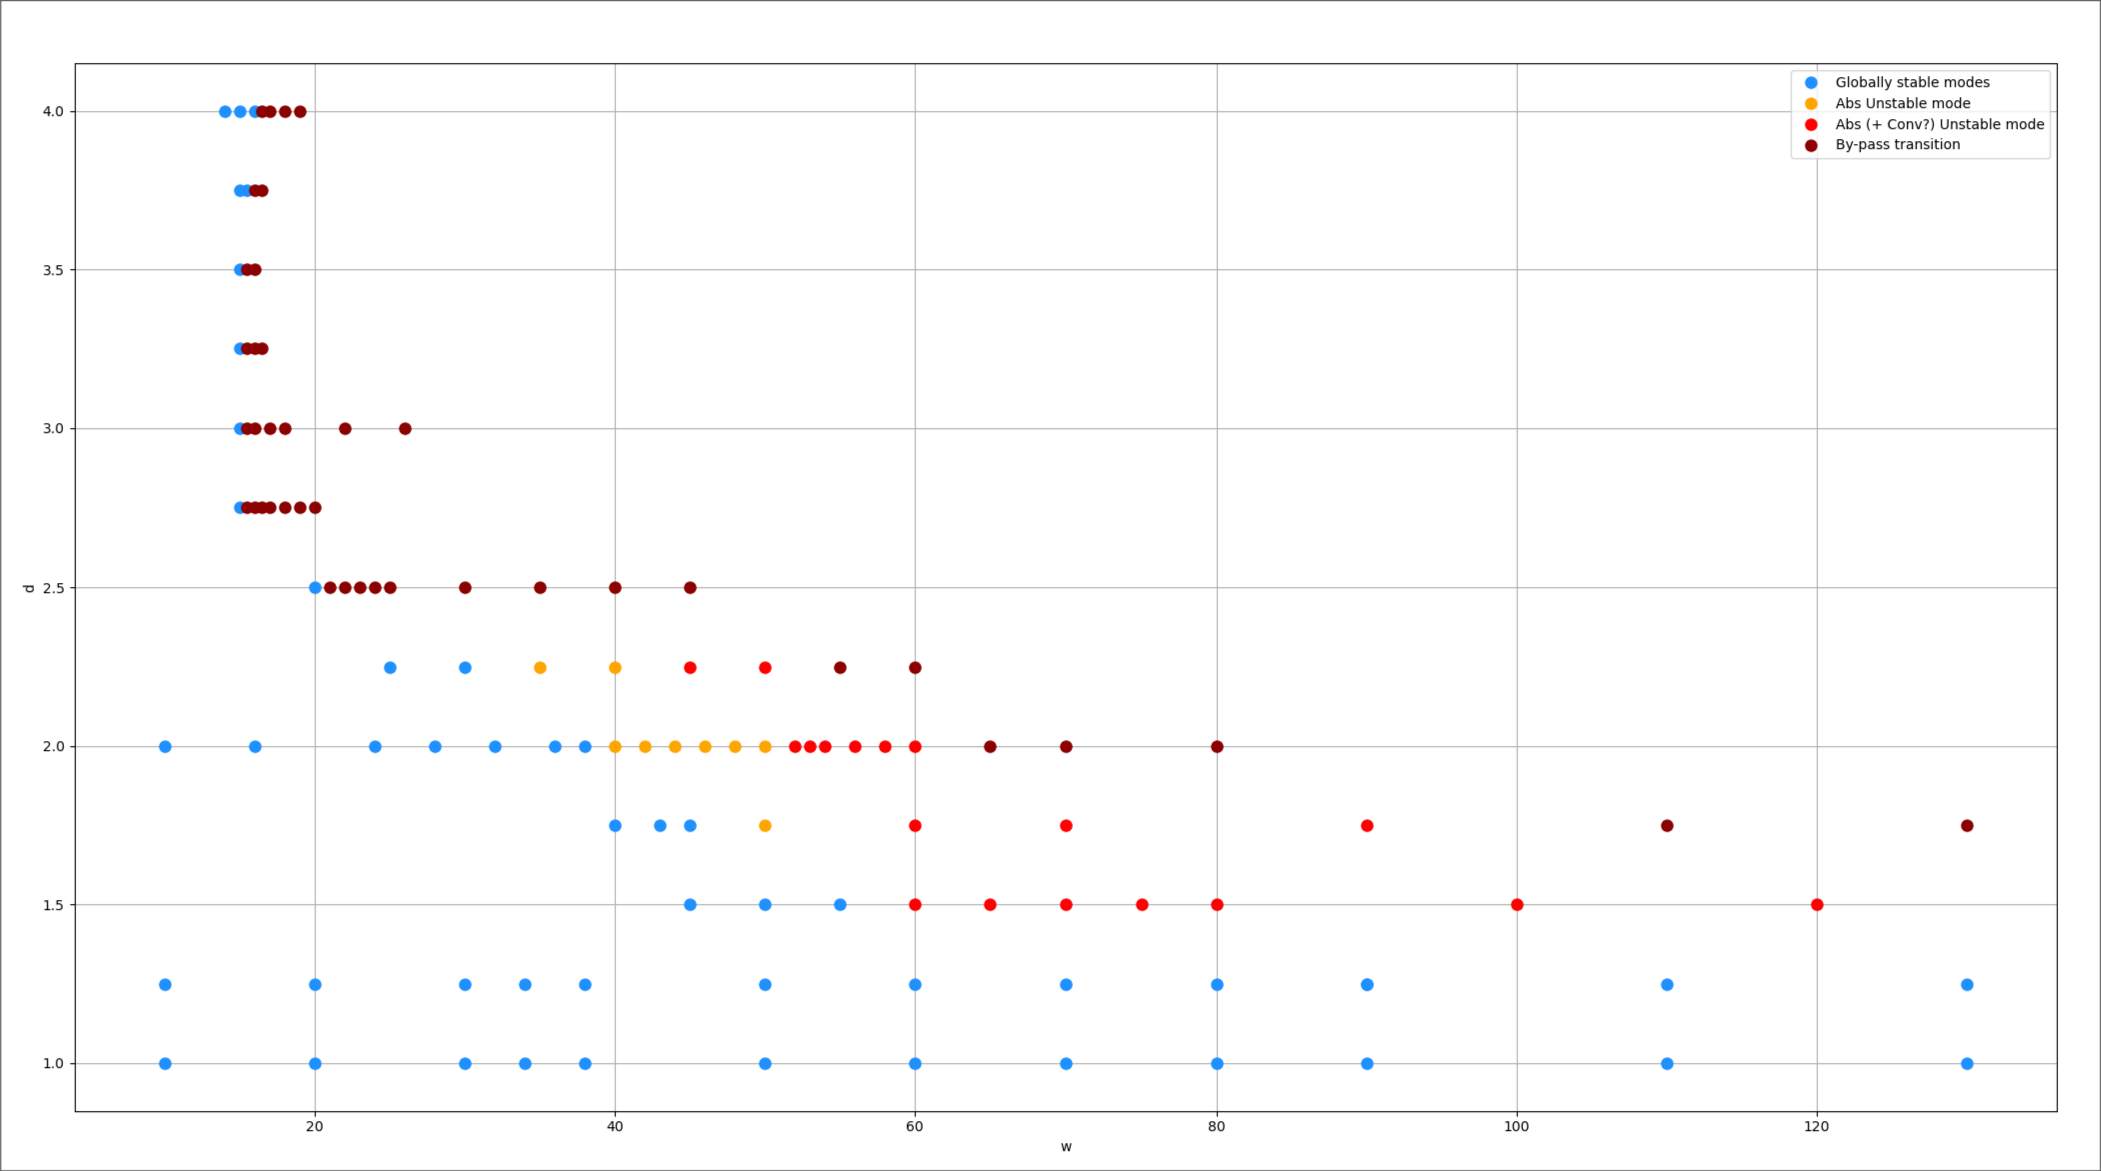
\includegraphics[width=0.8\linewidth]{Images/stabilitycurve.png}
\end{frame}
% At the end the parameters omega_r (= time frequency) and alpha_r (= wavelength) of the TS mode (from Orr-Sommerfeld eq) are correct and I am getting amplification in the amplitudes of the waves, as expected when blowing and suction. . I think last time I swapped them or anything even worse... Anyway the solver is correct. But in order to compute n(x) = max_omega m(x)

\begin{frame}
	\frametitle{Backward behaviour in $w$ in the stability line}
	\centering
	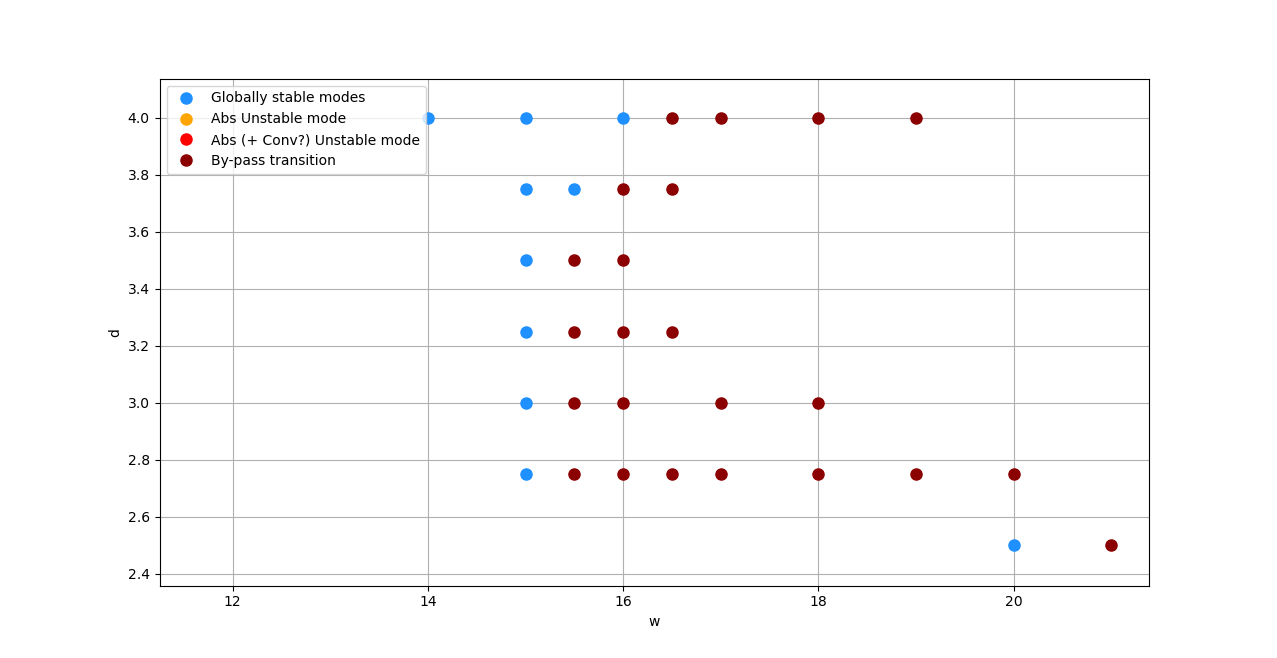
\includegraphics[width=0.7\linewidth]{Images/zoomedstabilitycurve.png}
\end{frame}
\begin{frame}
	\frametitle{$n(x)$ factor}
	\begin{itemize}
		\item Blowing-suction upstream as:
		      $$
			      v(x,t) = A \sin(\alpha_r(x - x_0))^3\sin(\omega_r t)\boldmath{1}_{x_0\leq x \leq x_0 + \ell}
		      $$
		      where $\ell=\pi/\alpha_r$, $A = 0.003$, $x_0 = -70\delta^*$, $\alpha_r = 0.1428, \omega_r = 0.04618$ (both from Orr-Sommerfeld eq).
	\end{itemize}
	$$
		n(x,\omega_r,\alpha_r) = \log\left(\frac{A^{TS}(x,\omega_r,\alpha_r)}{A_{0}^{TS}(\omega_r,\alpha_r)}\right)
	$$
	where $A^{TS}(x,\omega_r,\alpha_r)$ is the amplitude of the TS mode at $x$ and $A_{0}^{TS}(\omega_r,\alpha_r)$ is the amplitude of the TS mode at $x=x_0$ (how to choose $x_0$?).

	And then $$N(x) = \max_{\omega,\alpha}n(x,\omega,\alpha)$$ It would be nice to have our $n(x,\omega_r,\alpha_r)$ as closest as possible to the $N(x)$. Having observed the huge importance of the $v$ component of the baseflow, do we need to try weakly non-parallel Orr-Sommerfeld?
\end{frame}
\begin{frame}
	\centering
	\begin{columns}[T] % [T] ensures correct vertical alignment
		\begin{column}{0.6\linewidth} % Left column
			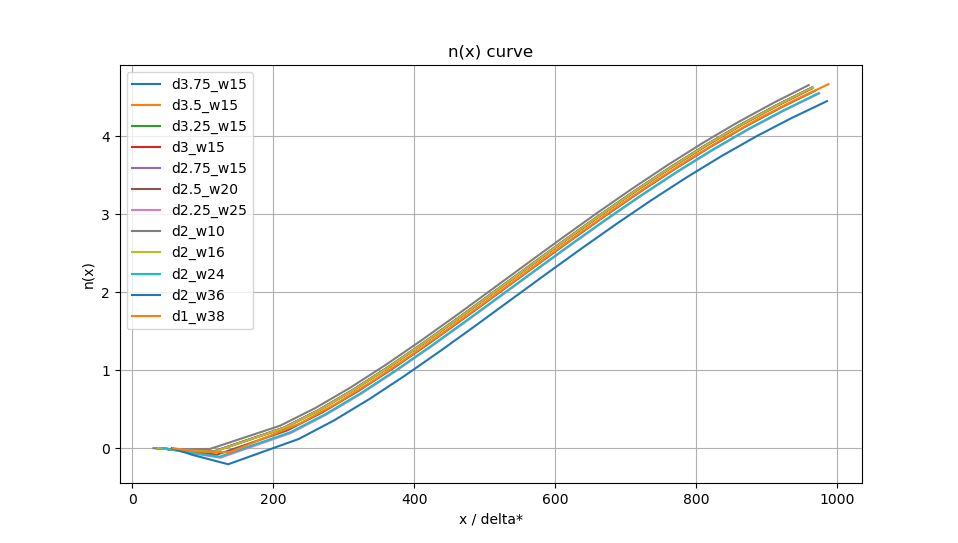
\includegraphics[width=\linewidth]{Images/nfactorCurve.png}
		\end{column}
		\begin{column}{0.38\linewidth} % Left column
			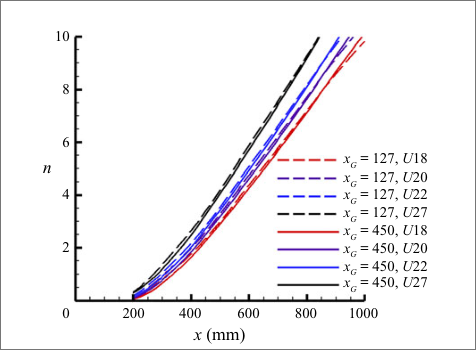
\includegraphics[width=\textwidth]{Images/jeffn.png}
		\end{column}
	\end{columns}
\end{frame}
\begin{frame}
	\frametitle{jeff $\Delta N$}

	\centering
	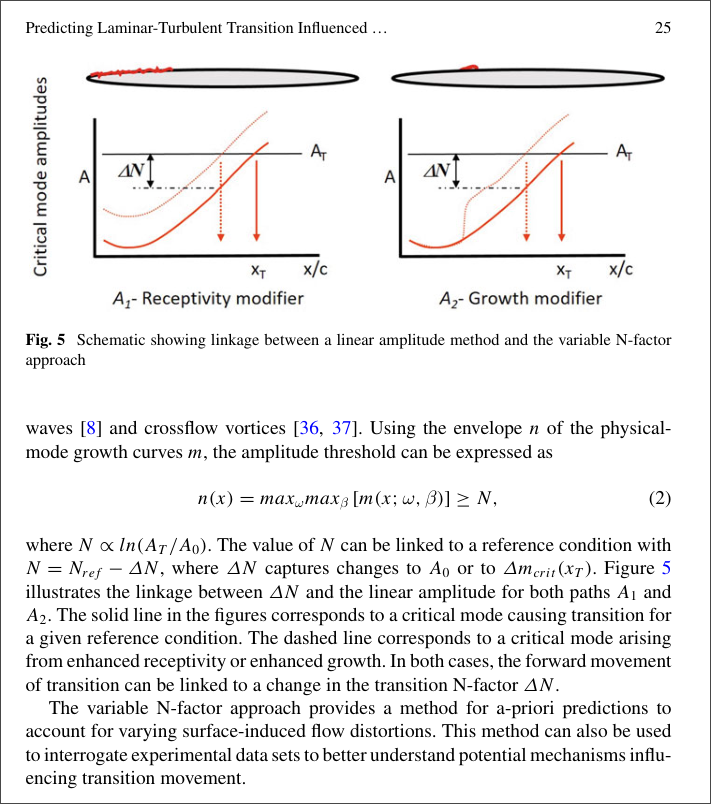
\includegraphics[width=0.5\linewidth]{Images/jeffPaper.png}
  
\end{frame}
\end{document}
